% answers.tex —— 2009 年·普通高等学校招生考试·重庆卷·文科 · 参考答案与详细解析片段
% 由 tools/generate_projects.py 依来源总账自 2009/2009_数学真题_重庆文_试题.md + 2009/2009_数学真题_重庆文_解析正文.md + 2009/2009_数学真题_重庆文_答案要点.md 生成，勿手改（改源 MD 后重跑）


\begin{gktip}
固定候选 PDF 仅含题面，无答案、解析和评分标准，原页亦未标分值；以下为非官方编者独立推导，官方答案字段为空。分数、根号、上下标与两幅图均以 600 dpi 原页复核。原页第 16 题第（1）问作「求 $\omega$ 的最小正周期」，$\omega$ 本身没有周期，按题面给出的最小正周期 $\dfrac{2\pi}3$ 理解为「求 $\omega$ 及函数的最小正周期」。
\end{gktip}

\begin{answer}
\gksolhead{1}{}

\textbf{题目}：

圆心在 $y$ 轴上，半径为 $1$，且过点 $(1,2)$ 的圆的方程为（　）

（A）$x^2+(y-2)^2=1$

（B）$x^2+(y+2)^2=1$

（C）$(x-1)^2+(y-3)^2=1$

（D）$x^2+(y-3)^2=1$

\Needspace{4\baselineskip}
\textbf{解析}

\Needspace{5\baselineskip}
设圆心为 $(0,k)$，由半径 $1$ 且过 $(1,2)$：

\nopagebreak[4]
\[(1-0)^2+(2-k)^2=1,\qquad (2-k)^2=0,\qquad k=2.\]

故圆的方程为 $x^2+(y-2)^2=1$。

\gkanswer{答案：A。}

\end{answer}
\begin{answer}
\gksolhead{2}{}

\textbf{题目}：

命题“若一个数是负数，则它的平方是正数”的逆命题是（　）

（A）“若一个数是负数，则它的平方不是正数”

（B）“若一个数的平方是正数，则它是负数”

（C）“若一个数不是负数，则它的平方不是正数”

（D）“若一个数的平方不是正数，则它不是负数”

\Needspace{4\baselineskip}
\textbf{解析}

原命题的条件是「一个数是负数」，结论是「它的平方是正数」。逆命题交换条件与结论：「若一个数的平方是正数，则它是负数」。

\gkanswer{答案：B。}

\end{answer}
\begin{answer}
\gksolhead{3}{}

\textbf{题目}：

$(x+2)^6$ 的展开式中 $x^3$ 的系数是（　）

（A）$20$

（B）$40$

（C）$80$

（D）$160$

\Needspace{4\baselineskip}
\textbf{解析}

\Needspace{5\baselineskip}
$(x+2)^6$ 的通项为 $\mathrm C_6^k x^{6-k}2^k$。令 $6-k=3$，得 $k=3$，系数为

\nopagebreak[4]
\[\mathrm C_6^3\cdot2^3=20\times8=160.\]

\gkanswer{答案：D。}

\end{answer}
\begin{answer}
\gksolhead{4}{}

\textbf{题目}：

已知向量 $\boldsymbol a=(1,1)$，$\boldsymbol b=(2,x)$．若 $\boldsymbol a+\boldsymbol b$ 与 $4\boldsymbol b-2\boldsymbol a$ 平行，则实数 $x$ 的值是（　）

（A）$-2$

（B）$0$

（C）$1$

（D）$2$

\Needspace{4\baselineskip}
\textbf{解析}

\nopagebreak[4]
\[\boldsymbol a+\boldsymbol b=(3,1+x),\qquad 4\boldsymbol b-2\boldsymbol a=(8-2,4x-2)=(6,4x-2).\]

\Needspace{5\baselineskip}
两向量平行，故

\nopagebreak[4]
\[3(4x-2)=6(1+x),\]

即 $12x-6=6+6x$，$x=2$。

\gkanswer{答案：D。}

\end{answer}
\begin{answer}
\gksolhead{5}{}

\textbf{题目}：

设 $\{a_n\}$ 是公差不为 $0$ 的等差数列，$a_1=2$ 且 $a_1$，$a_3$，$a_6$ 成等比数列，则 $\{a_n\}$ 的前 $n$ 项和 $S_n=$（　）

（A）$\dfrac{n^2}4+\dfrac{7n}4$

（B）$\dfrac{n^2}3+\dfrac{5n}3$

（C）$\dfrac{n^2}2+\dfrac{3n}4$

（D）$n^2+n$

\Needspace{4\baselineskip}
\textbf{解析}

\Needspace{5\baselineskip}
设公差为 $d\neq0$。$a_1=2$，$a_3=2+2d$，$a_6=2+5d$。由等比中项：

\nopagebreak[4]
\[(2+2d)^2=2(2+5d),\]

\nopagebreak[4]
\[4+8d+4d^2=4+10d,\qquad 4d^2-2d=0,\qquad d=\frac12.\]

\Needspace{5\baselineskip}
于是

\nopagebreak[4]
\[S_n=2n+\frac{n(n-1)}2\cdot\frac12=\frac{n^2+7n}4.\]

\gkanswer{答案：A。}

\end{answer}
\begin{answer}
\gksolhead{6}{}

\textbf{题目}：

下列关系式中正确的是（　）

（A）$\sin11^\circ<\cos10^\circ<\sin168^\circ$

（B）$\sin168^\circ<\sin11^\circ<\cos10^\circ$

（C）$\sin11^\circ<\sin168^\circ<\cos10^\circ$

（D）$\sin168^\circ<\cos10^\circ<\sin11^\circ$

\Needspace{4\baselineskip}
\textbf{解析}

\Needspace{5\baselineskip}
$\sin168^\circ=\sin(180^\circ-12^\circ)=\sin12^\circ$，$\cos10^\circ=\sin80^\circ$。三个角 $11^\circ<12^\circ<80^\circ$ 都在 $(0^\circ,90^\circ)$ 内，正弦函数递增，故

\nopagebreak[4]
\[\sin11^\circ<\sin168^\circ<\cos10^\circ.\]

\gkanswer{答案：C。}

\end{answer}
\begin{answer}
\gksolhead{7}{}

\textbf{题目}：

已知 $a>0$，$b>0$，则 $\dfrac1a+\dfrac1b+2\sqrt{ab}$ 的最小值是（　）

（A）$2$

（B）$2\sqrt2$

（C）$4$

（D）$5$

\Needspace{4\baselineskip}
\textbf{解析}

\Needspace{5\baselineskip}
由基本不等式 $\dfrac1a+\dfrac1b\geqslant\dfrac2{\sqrt{ab}}$。令 $t=\sqrt{ab}>0$，则

\nopagebreak[4]
\[\frac1a+\frac1b+2\sqrt{ab}\geqslant\frac2t+2t\geqslant2\sqrt{\frac2t\cdot2t}=4,\]

当 $a=b=1$ 时取等号。故最小值为 $4$。

\gkanswer{答案：C。}

\end{answer}
\begin{answer}
\gksolhead{8}{}

\textbf{题目}：

$12$ 个篮球队中有 $3$ 个强队，将这 $12$ 个队任意分成 $3$ 个组（每组 $4$ 个队），则 $3$ 个强队恰好被分在同一组的概率为（　）

（A）$\dfrac1{55}$

（B）$\dfrac3{55}$

（C）$\dfrac14$

（D）$\dfrac13$

\Needspace{4\baselineskip}
\textbf{解析}

\Needspace{5\baselineskip}
先固定一个强队，它所在的组还有 $3$ 个名额，从其余 $11$ 个队中选。另两个强队都进入该组的概率为

\nopagebreak[4]
\[\frac3{11}\cdot\frac2{10}=\frac3{55}.\]

\gkanswer{答案：B。}

\end{answer}
\begin{answer}
\gksolhead{9}{}

\textbf{题目}：

在正四棱柱 $ABCD-A_1B_1C_1D_1$ 中，顶点 $B_1$ 到对角线 $BD_1$ 和到平面 $A_1BCD_1$ 的距离分别为 $h$ 和 $d$，则下列命题中正确的是（　）

（A）若侧棱的长小于底面的边长，则 $\dfrac hd$ 的取值范围为 $(0,1)$

（B）若侧棱的长小于底面的边长，则 $\dfrac hd$ 的取值范围为 $\left(\dfrac{\sqrt2}2,\dfrac{2\sqrt3}3\right)$

（C）若侧棱的长大于底面的边长，则 $\dfrac hd$ 的取值范围为 $\left(\dfrac{2\sqrt3}3,\sqrt2\right)$

（D）若侧棱的长大于底面的边长，则 $\dfrac hd$ 的取值范围为 $\left(\dfrac{2\sqrt3}3,+\infty\right)$

\Needspace{4\baselineskip}
\textbf{解析}

\Needspace{5\baselineskip}
设底面边长 $a$，侧棱长 $b$。取坐标 $B(a,0,0)$，$D_1(0,a,b)$，则

\nopagebreak[4]
\[h=\frac{\sqrt2ab}{\sqrt{2a^2+b^2}},\qquad d=\frac{ab}{\sqrt{a^2+b^2}}.\]

\Needspace{5\baselineskip}
故

\nopagebreak[4]
\[\frac hd=\sqrt{\frac{2(a^2+b^2)}{2a^2+b^2}}.\]

令 $t=\dfrac ba$。当 $0<t<1$ 时，$\dfrac hd$ 从 $1$ 递增到 $\dfrac{2\sqrt3}3$，取值范围为 $\left(1,\dfrac{2\sqrt3}3\right)$，故（A）（B）均错；当 $t>1$ 时，$\dfrac hd$ 继续递增，$t\to+\infty$ 时趋于 $\sqrt2$，取值范围为 $\left(\dfrac{2\sqrt3}3,\sqrt2\right)$，故（C）正确，（D）错。

\gkanswer{答案：C。}

\end{answer}
\begin{answer}
\gksolhead{10}{}

\textbf{题目}：

把函数 $f(x)=x^3-3x$ 的图象 $C_1$ 向右平移 $u$ 个单位长度，再向下平移 $v$ 个单位长度后得到图象 $C_2$．若对任意的 $u>0$，曲线 $C_1$ 与 $C_2$ 至多只有一个交点，则 $v$ 的最小值为（　）

（A）$2$

（B）$4$

（C）$6$

（D）$8$

\Needspace{4\baselineskip}
\textbf{解析}

\Needspace{5\baselineskip}
平移后 $C_2:y=(x-u)^3-3(x-u)-v$。与 $C_1:y=x^3-3x$ 联立，化简得

\nopagebreak[4]
\[x^2-ux+\frac{u^2-3}3+\frac v{3u}=0.\]

\Needspace{5\baselineskip}
对任意 $u>0$ 至多一个交点，判别式须非正：

\nopagebreak[4]
\[\Delta=u^2-4\left(\frac{u^2-3}3+\frac v{3u}\right)\leqslant0,\]

即 $v\geqslant\dfrac{u(12-u^2)}4$ 对一切 $u>0$ 成立。右端最大值在 $u=2$ 时取得，为 $4$。故 $v$ 的最小值为 $4$。

\gkanswer{答案：B。}

\end{answer}
\begin{answer}
\gksolhead{11}{}

\textbf{题目}：

若 $U=\{n\mid n\text{ \text{是小于} }9\text{ \text{的正整数}}\}$，$A=\{n\in U\mid n\text{ \text{是奇数}}\}$，$B=\{n\in U\mid n\text{ \text{是} }3\text{ \text{的倍数}}\}$，则 $\complement_U(A\cup B)=$ $\underline{\qquad}$．

\Needspace{4\baselineskip}
\textbf{解析}

\Needspace{5\baselineskip}
$U=\{1,2,\ldots,8\}$，$A=\{1,3,5,7\}$，$B=\{3,6\}$，故 $A\cup B=\{1,3,5,6,7\}$，

\nopagebreak[4]
\[\complement_U(A\cup B)=\{2,4,8\}.\]

\gkanswer{答案：$\{2,4,8\}$。}

\end{answer}
\begin{answer}
\gksolhead{12}{}

\textbf{题目}：

记 $f(x)=\log_3(x+1)$ 的反函数为 $y=f^{-1}(x)$，则方程 $f^{-1}(x)=8$ 的解 $x=$ $\underline{\qquad}$．

\Needspace{4\baselineskip}
\textbf{解析}

由 $y=\log_3(x+1)$ 得 $x+1=3^y$，故 $f^{-1}(x)=3^x-1$。令 $3^x-1=8$，得 $3^x=9$，$x=2$。

\gkanswer{答案：$2$。}

\end{answer}
\begin{answer}
\gksolhead{13}{}

\textbf{题目}：

$5$ 个人站成一排，其中甲、乙两人不相邻的排法有$\underline{\qquad}$种．（用数字作答）

\Needspace{4\baselineskip}
\textbf{解析}

\Needspace{5\baselineskip}
$5$ 人全排列共 $5!=120$ 种。甲、乙相邻时把两人捆成一组，有 $2\times4!=48$ 种。故不相邻的排法为

\nopagebreak[4]
\[120-48=72.\]

\gkanswer{答案：$72$。}

\end{answer}
\begin{answer}
\gksolhead{14}{}

\textbf{题目}：

\Needspace{5\baselineskip}
从一堆苹果中任取 $5$ 只，称得它们的质量如下（单位：克）：

\nopagebreak[4]
\[125\quad 124\quad 121\quad 123\quad 127\]

则该样本标准差 $s=$ $\underline{\qquad}$（克）．（用数字作答）

\Needspace{4\baselineskip}
\textbf{解析}

\Needspace{5\baselineskip}
平均值

\nopagebreak[4]
\[\bar x=\frac{125+124+121+123+127}5=124.\]

\Needspace{5\baselineskip}
样本方差

\nopagebreak[4]
\[s^2=\frac{(1)^2+0^2+(-3)^2+(-1)^2+3^2}{5-1}=\frac{20}4=5,\]

故 $s=\sqrt5$。

\gkanswer{答案：$\sqrt5$。}

\end{answer}
\begin{answer}
\gksolhead{15}{}

\textbf{题目}：

已知椭圆 $\dfrac{x^2}{a^2}+\dfrac{y^2}{b^2}=1$（$a>b>0$）的左、右焦点分别为 $F_1(-c,0)$，$F_2(c,0)$．若椭圆上存在一点 $P$ 使 $\dfrac a{\sin\angle PF_1F_2}=\dfrac c{\sin\angle PF_2F_1}$，则该椭圆的离心率的取值范围为$\underline{\qquad}$．

\Needspace{4\baselineskip}
\textbf{解析}

\Needspace{5\baselineskip}
在 $\triangle PF_1F_2$ 中，由正弦定理

\nopagebreak[4]
\[\frac{PF_2}{\sin\angle PF_1F_2}=\frac{PF_1}{\sin\angle PF_2F_1}.\]

\Needspace{5\baselineskip}
结合题设 $\dfrac a{\sin\angle PF_1F_2}=\dfrac c{\sin\angle PF_2F_1}$，得

\nopagebreak[4]
\[\frac{PF_1}{PF_2}=\frac ca=e.\]

\Needspace{5\baselineskip}
又 $PF_1+PF_2=2a$，故 $PF_1=\dfrac{2ae}{1+e}$，$PF_2=\dfrac{2a}{1+e}$。椭圆上点的焦半径范围为 $[a-c,a+c]$，于是

\nopagebreak[4]
\[\frac{1-e}{1+e}\leqslant e\leqslant\frac{1+e}{1-e}.\]

右端对 $0<e<1$ 恒成立；左端化为 $e^2+2e-1\geqslant0$，即 $e\geqslant\sqrt2-1$。故 $e\in[\sqrt2-1,1)$。

\gkanswer{答案：$[\sqrt2-1,1)$。}

\end{answer}
\begin{answer}
\gksolhead{16}{}

\textbf{题目}：

设函数 $f(x)=(\sin\omega x+\cos\omega x)^2+2\cos^2\omega x$（$\omega>0$）的最小正周期为 $\dfrac{2\pi}3$．

（1）求 $\omega$ 的最小正周期；

（2）若函数 $y=g(x)$ 的图象是由 $y=f(x)$ 的图象向右平移 $\dfrac\pi2$ 个单位长度得到，求 $y=g(x)$ 的单调增区间．

\Needspace{4\baselineskip}
\textbf{解析}

\Needspace{5\baselineskip}
（1）

\nopagebreak[4]
\[f(x)=1+\sin2\omega x+1+\cos2\omega x=2+\sqrt2\sin\left(2\omega x+\frac\pi4\right).\]

最小正周期 $\dfrac{2\pi}{2\omega}=\dfrac\pi\omega=\dfrac{2\pi}3$，故 $\omega=\dfrac32$。原页「求 $\omega$ 的最小正周期」表述有误，$\omega$ 无周期，按题意同时给出 $\omega$ 与函数的最小正周期。

\Needspace{5\baselineskip}
（2）将 $f(x)=2+\sqrt2\sin\left(3x+\dfrac\pi4\right)$ 向右平移 $\dfrac\pi2$：

\nopagebreak[4]
\[g(x)=2+\sqrt2\sin\left(3\left(x-\frac\pi2\right)+\frac\pi4\right)
=2+\sqrt2\sin\left(3x-\frac{5\pi}4\right).\]

\Needspace{5\baselineskip}
令 $3x-\dfrac{5\pi}4\in\left[-\dfrac\pi2+2k\pi,\dfrac\pi2+2k\pi\right]$，得

\nopagebreak[4]
\[3x\in\left[\frac{3\pi}4+2k\pi,\frac{7\pi}4+2k\pi\right],\]

\nopagebreak[4]
\[x\in\left[\frac\pi4+\frac{2k\pi}3,\frac{7\pi}{12}+\frac{2k\pi}3\right],\qquad k\in\mathbf Z.\]

\gkanswer{答案：（1）$\omega=\dfrac32$，最小正周期 $\dfrac{2\pi}3$；（2）$\left[\dfrac\pi4+\dfrac{2k\pi}3,\dfrac{7\pi}{12}+\dfrac{2k\pi}3\right]$，$k\in\mathbf Z$。}

\end{answer}
\begin{answer}
\gksolhead{17}{}

\textbf{题目}：

某单位为绿化环境，移栽了甲、乙两种大树各 $2$ 株．设甲、乙两种大树移栽的成活率分别为 $\dfrac56$ 和 $\dfrac45$，且各株大树是否成活互不影响．求移栽的 $4$ 株大树中：

（1）至少有 $1$ 株成活的概率；

（2）两种大树各成活 $1$ 株的概率．

\Needspace{4\baselineskip}
\textbf{解析}

\Needspace{5\baselineskip}
（1）各株不成活的概率分别为 $\dfrac16$，$\dfrac15$，且相互独立。四株全不成活的概率为

\nopagebreak[4]
\[\left(\frac16\right)^2\left(\frac15\right)^2=\frac1{900},\]

故至少一株成活的概率为 $1-\dfrac1{900}=\dfrac{899}{900}$。

\Needspace{5\baselineskip}
（2）甲种树恰成活 $1$ 株的概率为

\nopagebreak[4]
\[\mathrm C_2^1\cdot\frac56\cdot\frac16=\frac{10}{36}=\frac5{18};\]

\Needspace{5\baselineskip}
乙种树恰成活 $1$ 株的概率为

\nopagebreak[4]
\[\mathrm C_2^1\cdot\frac45\cdot\frac15=\frac8{25}.\]

\Needspace{5\baselineskip}
两事件独立，故所求概率为

\nopagebreak[4]
\[\frac5{18}\cdot\frac8{25}=\frac4{45}.\]

\gkanswer{答案：（1）$\dfrac{899}{900}$；（2）$\dfrac4{45}$。}

\end{answer}
\begin{answer}
\gksolhead{18}{}

\textbf{题目}：

如图，在五面体 $ABCDEF$ 中，$AB\parallel DC$，$\angle BAD=\dfrac\pi2$，$CD=AD=2$，四边形 $ABFE$ 为平行四边形，$FA\perp$ 平面 $ABCD$，$FC=3$，$ED=\sqrt7$．求：

（1）直线 $AB$ 到平面 $EFCD$ 的距离；

（2）二面角 $F-AD-E$ 的平面角的正切值．
\nopagebreak[4]
\begin{center}% 2009 年重庆卷文科第 18 题：五面体 ABCDEF（AB∥DC，FA⊥平面 ABCD，ABFE 为平行四边形）。
% 来源 PDF：普通高考/2009/2009重庆文.pdf，SHA-256 c4d433586be8144d34c8ee2d4074c6308f53ffe84aa3a8a7ea28bb6f0cf86a39。
% 原页：第 1 页（A3 三栏）第 3 栏下部，书页码 505。
% 重绘依据：由题设取 A(0,0,0)、B(-√2,0,0)、D(0,2,0)、C(-2,2,0)、F(0,0,1)、E(√2,0,1)。
%   可见外轮廓 F-E-D-C-B-F 为实线；FA、AB、AD 为被遮挡或内部辅助线，画虚线。
%   投影取 (x,y,z) -> (x+0.35y, 2.20z+0.28y)。
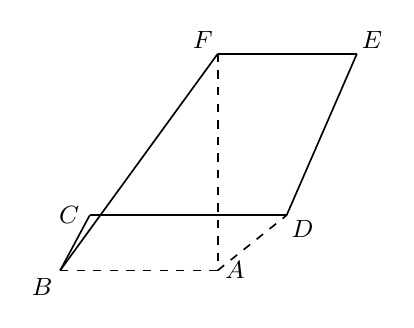
\begin{tikzpicture}[semithick, scale=1.25, every node/.style={inner sep=1.5pt, font=\small}]
  \coordinate (A) at (0.000,0.000);
  \coordinate (B) at (-1.600,0.000);
  \coordinate (C) at (-1.300,0.560);
  \coordinate (D) at (0.700,0.560);
  \coordinate (F) at (0.000,2.200);
  \coordinate (E) at (1.414,2.200);

  % 外轮廓
  \draw (F) -- (E);
  \draw (E) -- (D);
  \draw (D) -- (C);
  \draw (C) -- (B);
  \draw (B) -- (F);

  % 内部与遮挡线
  \draw[dashed] (F) -- (A);
  \draw[dashed] (A) -- (B);
  \draw[dashed] (A) -- (D);

  % 标注
  \node[right=1pt] at (A) {$A$};
  \node[below left=1pt] at (B) {$B$};
  \node[left=2pt] at (C) {$C$};
  \node[below right] at (D) {$D$};
  \node[above left] at (F) {$F$};
  \node[above right] at (E) {$E$};
\end{tikzpicture}
\end{center}
\nopagebreak[4]
\Needspace{4\baselineskip}
\textbf{解析}

\Needspace{5\baselineskip}
（1）以 $A$ 为原点，$AD$ 为 $y$ 轴，$AB$ 的反方向为 $x$ 轴，$AF$ 为 $z$ 轴建系。设 $AF=h$，$AB=b$，则

\nopagebreak[4]
\[A(0,0,0),\ B(-b,0,0),\ D(0,2,0),\ C(-2,2,0),\ F(0,0,h).\]

\Needspace{5\baselineskip}
由 $FC=3$：

\nopagebreak[4]
\[(-2)^2+2^2+h^2=9,\qquad h=1.\]

\Needspace{5\baselineskip}
由 $ED=\sqrt7$，且 $ABFE$ 为平行四边形，$E=A+F-B=(b,0,1)$：

\nopagebreak[4]
\[b^2+2^2+1^2=7,\qquad b=\sqrt2.\]

\Needspace{5\baselineskip}
平面 $EFCD$ 过 $E(\sqrt2,0,1)$，$F(0,0,1)$，$C(-2,2,0)$，$D(0,2,0)$，其方程为 $y+2z-2=0$。直线 $AB$ 在 $y=z=0$ 上，方向与平面平行，故距离为

\nopagebreak[4]
\[\frac{|0+0-2|}{\sqrt{1^2+2^2}}=\frac2{\sqrt5}=\frac{2\sqrt5}5.\]

\Needspace{5\baselineskip}
（2）平面 $FAD$ 的法向量为 $(1,0,0)$。平面 $EAD$ 由 $\overrightarrow{AD}=(0,2,0)$ 与 $\overrightarrow{AE}=(\sqrt2,0,1)$ 张成，法向量

\nopagebreak[4]
\[\boldsymbol n=(0,2,0)\times(\sqrt2,0,1)=(2,0,-2\sqrt2),\]

\Needspace{5\baselineskip}
取 $(1,0,-\sqrt2)$。设二面角为 $\theta$，则

\nopagebreak[4]
\[\cos\theta=\frac{|(1,0,0)\cdot(1,0,-\sqrt2)|}{1\cdot\sqrt3}=\frac1{\sqrt3},\]

故 $\tan\theta=\sqrt2$。

\gkanswer{答案：（1）$\dfrac{2\sqrt5}5$；（2）$\sqrt2$。}

\end{answer}
\begin{answer}
\gksolhead{19}{}

\textbf{题目}：

已知 $f(x)=x^2+bx+c$ 为偶函数，曲线 $y=f(x)$ 过点 $(2,5)$，$g(x)=(x+a)f(x)$．

（1）若曲线 $y=g(x)$ 有斜率为 $0$ 的切线，求实数 $a$ 的取值范围；

（2）若当 $x=-1$ 时函数 $y=g(x)$ 取得极值，确定 $y=g(x)$ 的单调区间．

\Needspace{4\baselineskip}
\textbf{解析}

\Needspace{5\baselineskip}
（1）$f(x)$ 为偶函数，故 $b=0$。又 $f(2)=5$，即 $4+c=5$，$c=1$，故 $f(x)=x^2+1$，

\nopagebreak[4]
\[g(x)=(x+a)(x^2+1)=x^3+ax^2+x+a.\]

\Needspace{5\baselineskip}
曲线有斜率为 $0$ 的切线，即 $g'(x)=3x^2+2ax+1$ 有实根：

\nopagebreak[4]
\[\Delta=4a^2-12\geqslant0,\qquad a^2\geqslant3.\]

故 $a\leqslant-\sqrt3$ 或 $a\geqslant\sqrt3$。

\Needspace{5\baselineskip}
（2）$x=-1$ 为极值点，故

\nopagebreak[4]
\[g'(-1)=3-2a+1=0,\qquad a=2.\]

此时 $g'(x)=3x^2+4x+1=(3x+1)(x+1)$。由 $g'(x)>0$ 得 $x<-1$ 或 $x>-\dfrac13$；由 $g'(x)<0$ 得 $-1<x<-\dfrac13$。故增区间为 $(-\infty,-1)$ 与 $\left(-\dfrac13,+\infty\right)$，减区间为 $\left(-1,-\dfrac13\right)$。

\gkanswer{答案：（1）$a\leqslant-\sqrt3$ 或 $a\geqslant\sqrt3$；（2）增区间 $(-\infty,-1)$，$\left(-\dfrac13,+\infty\right)$，减区间 $\left(-1,-\dfrac13\right)$。}

\end{answer}
\begin{answer}
\gksolhead{20}{}

\textbf{题目}：

已知以原点 $O$ 为中心的双曲线的一条准线方程为 $x=\dfrac{\sqrt5}5$，离心率 $e=\sqrt5$．

（1）求该双曲线的方程；

（2）如图，点 $A$ 的坐标为 $(-\sqrt5,0)$，$B$ 是圆 $x^2+(y-\sqrt5)^2=1$ 上的点，点 $M$ 在双曲线右支上，求 $|MA|+|MB|$ 的最小值，并求此时 $M$ 点的坐标．
\nopagebreak[4]
\begin{center}% 2009 年重庆卷文科第 20 题：双曲线右支、圆 x^2+(y-√5)^2=1 与点 A、B、M。
% 来源 PDF：普通高考/2009/2009重庆文.pdf，SHA-256 c4d433586be8144d34c8ee2d4074c6308f53ffe84aa3a8a7ea28bb6f0cf86a39。
% 原页：第 2 页（A3 三栏）第 2 栏上部，书页码 506。
% 重绘依据：按题设双曲线 x^2-y^2/4=1 与圆 x^2+(y-√5)^2=1 等比绘制；
%   A(-√5,0) 为左焦点，M 取右支上使 |MA|+|MB| 最小的点，B 取圆上相应点。
\begin{tikzpicture}[semithick, x=1.2cm, y=1.2cm, every node/.style={inner sep=1.5pt, font=\small}]
  % 坐标轴
  \draw[-stealth] (-3.0,0) -- (3.0,0) node[below] {$x$};
  \draw[-stealth] (0,-0.5) -- (0,4.0) node[left] {$y$};
  \node[below left] at (0,0) {$O$};

  % 双曲线右支
  \draw[domain=-2.3:2.3, samples=120, thick] plot ({sqrt(1+(\x*\x)/4)},{\x});

  % 圆
  \draw[thick] (0,2.236) circle (1);

  % 点与线段
  \coordinate (A) at (-2.236,0);
  \coordinate (B) at (0.707,1.529);
  \coordinate (M) at (1.140,1.096);
  \fill (A) circle (1.4pt);
  \fill (B) circle (1.4pt);
  \fill (M) circle (1.4pt);
  \draw (A) -- (M);
  \draw[dashed] (M) -- (B);

  % 标注
  \node[below left] at (A) {$A$};
  \node[above left] at (B) {$B$};
  \node[right] at (M) {$M$};
\end{tikzpicture}
\end{center}
\nopagebreak[4]
\Needspace{4\baselineskip}
\textbf{解析}

\Needspace{5\baselineskip}
（1）设双曲线为 $\dfrac{x^2}{a^2}-\dfrac{y^2}{b^2}=1$。准线 $x=\dfrac{a^2}c=\dfrac{\sqrt5}5$，又 $e=\dfrac ca=\sqrt5$，故 $\dfrac{a^2}c=\dfrac ae=\dfrac a{\sqrt5}=\dfrac{\sqrt5}5$，得 $a=1$，$c=\sqrt5$，$b^2=c^2-a^2=4$。方程为

\nopagebreak[4]
\[x^2-\frac{y^2}4=1.\]

\Needspace{5\baselineskip}
（2）双曲线左焦点为 $A(-\sqrt5,0)$，右焦点为 $F_2(\sqrt5,0)$。$M$ 在右支上，故

\nopagebreak[4]
\[|MA|-|MF_2|=2a=2,\qquad |MA|=|MF_2|+2.\]

\Needspace{5\baselineskip}
设圆圆心 $C(0,\sqrt5)$，半径 $1$。于是

\nopagebreak[4]
\[|MA|+|MB|=|MF_2|+|MB|+2\geqslant|BF_2|+2\geqslant|CF_2|-1+2.\]

\Needspace{5\baselineskip}
而 $|CF_2|=\sqrt{(\sqrt5)^2+(\sqrt5)^2}=\sqrt{10}$，故

\nopagebreak[4]
\[|MA|+|MB|\geqslant\sqrt{10}+1.\]

\Needspace{5\baselineskip}
等号成立当 $B$ 在线段 $CF_2$ 上且 $M$ 在线段 $BF_2$ 上，即 $M$ 为线段 $CF_2$ 与双曲线右支的交点。令 $M=F_2+t(C-F_2)$，$0\leqslant t\leqslant1$，则

\nopagebreak[4]
\[x=\sqrt5(1-t),\qquad y=\sqrt5t.\]

\Needspace{5\baselineskip}
代入双曲线方程：

\nopagebreak[4]
\[5(1-t)^2-\frac{5t^2}4=1,\]

\nopagebreak[4]
\[20(1-2t+t^2)-5t^2=4,\qquad 15t^2-40t+16=0,\]

\nopagebreak[4]
\[t=\frac{20-4\sqrt{10}}{15}.\]

\Needspace{5\baselineskip}
故

\nopagebreak[4]
\[x=\frac{4\sqrt2-\sqrt5}3,\qquad y=\frac{4(\sqrt5-\sqrt2)}3.\]

此时 $|MA|+|MB|=\sqrt{10}+1$。

\gkanswer{答案：（1）$x^2-\dfrac{y^2}4=1$；（2）$\sqrt{10}+1$，$M\left(\dfrac{4\sqrt2-\sqrt5}3,\dfrac{4(\sqrt5-\sqrt2)}3\right)$。}

\end{answer}
\begin{answer}
\gksolhead{21}{}

\textbf{题目}：

已知 $a_1=1$，$a_2=4$，$a_{n+2}=4a_{n+1}+a_n$，$b_n=\dfrac{a_{n+1}}{a_n}$，$n\in\mathbf N^*$．

（1）求 $b_1$，$b_2$，$b_3$ 的值；

（2）设 $c_n=b_nb_{n+1}$，$S_n$ 为数列 $\{c_n\}$ 的前 $n$ 项和，求证：$S_n\geqslant17n$；

（3）求证：$|b_{2n}-b_n|<\dfrac1{64}\cdot\dfrac1{17^{n-2}}$．

\Needspace{4\baselineskip}
\textbf{解析}

\Needspace{5\baselineskip}
（1）$a_3=4a_2+a_1=17$，$a_4=4a_3+a_2=72$，故

\nopagebreak[4]
\[b_1=\frac{a_2}{a_1}=4,\qquad b_2=\frac{a_3}{a_2}=\frac{17}4,\qquad b_3=\frac{a_4}{a_3}=\frac{72}{17}.\]

\Needspace{5\baselineskip}
（2）由 $b_n=\dfrac{a_{n+1}}{a_n}$，

\nopagebreak[4]
\[b_{n+1}=\frac{a_{n+2}}{a_{n+1}}=\frac{4a_{n+1}+a_n}{a_{n+1}}=4+\frac1{b_n}.\]

\Needspace{5\baselineskip}
于是

\nopagebreak[4]
\[c_n=b_nb_{n+1}=b_n\left(4+\frac1{b_n}\right)=4b_n+1.\]

\Needspace{5\baselineskip}
由 $b_1=4$ 及 $b_{n+1}=4+\dfrac1{b_n}>4$，得 $b_n\geqslant4$，故 $c_n\geqslant17$，

\nopagebreak[4]
\[S_n=c_1+c_2+\cdots+c_n\geqslant17n.\]

\Needspace{5\baselineskip}
（3）令 $L=2+\sqrt5$，它是 $x=4+\dfrac1x$ 的正根，且 $L^2=9+4\sqrt5>17$。由

\nopagebreak[4]
\[b_{n+1}-L=\frac{L-b_n}{b_nL}=-\frac{b_n-L}{b_nL},\]

\Needspace{5\baselineskip}
对 $n\geqslant2$，由 $b_n=4+\dfrac1{b_{n-1}}$ 及 $4<b_n\leqslant\dfrac{17}4$ 归纳得 $b_n\geqslant b_3=\dfrac{72}{17}$，于是

\nopagebreak[4]
\[b_nL\geqslant\frac{72}{17}(2+\sqrt5)>17,\]

\Needspace{5\baselineskip}
从而

\nopagebreak[4]
\[|b_{n+1}-L|<\frac1{17}|b_n-L|.\]

\Needspace{5\baselineskip}
于是对 $n\geqslant2$，

\nopagebreak[4]
\[|b_n-L|\leqslant\frac{|b_2-L|}{17^{n-2}},\qquad
|b_{2n}-L|\leqslant\frac{|b_2-L|}{17^{2n-2}}.\]

\Needspace{5\baselineskip}
由三角不等式，

\nopagebreak[4]
\[|b_{2n}-b_n|\leqslant|b_{2n}-L|+|b_n-L|
\leqslant\frac{|b_2-L|}{17^{n-2}}\left(1+\frac1{17^n}\right).\]

\Needspace{5\baselineskip}
而

\nopagebreak[4]
\[|b_2-L|=\frac{17}4-(2+\sqrt5)=\frac94-\sqrt5<\frac1{70},\]

\Needspace{5\baselineskip}
且

\nopagebreak[4]
\[\frac1{70}\left(1+\frac1{289}\right)=\frac{29}{2023}<\frac1{64},\]

\Needspace{5\baselineskip}
故对 $n\geqslant2$，

\nopagebreak[4]
\[|b_{2n}-b_n|<\frac1{64}\cdot\frac1{17^{n-2}}.\]

\Needspace{5\baselineskip}
$n=1$ 时直接验证：

\nopagebreak[4]
\[|b_2-b_1|=\frac{17}4-4=\frac14<\frac{17}{64}=\frac1{64}\cdot\frac1{17^{-1}}.\]

综上，对一切 $n\in\mathbf N^*$ 不等式成立。

\gkanswer{答案：（1）$b_1=4$，$b_2=\dfrac{17}4$，$b_3=\dfrac{72}{17}$；（2）证明见解析；（3）证明见解析。}

\end{answer}